\section{Results}
\Cref{table:Average-metric-dataset-1} shows the mean metrics accross
all the time series in dataset 1. The poorest perfoming model accross the board
is SARIMA, with a MASE of $1.294$, sMAPE of $0.239$ and 7 day MASE of $1.063$.
All the different LSTM structures and hybrid methods outperformed SARIMA.

The multivariate models outperformed all the
%% Globale metoder gjør det bedre enn locale på MASE, men dårligere på sMAPE
% Kan det være fordi sMAPE straffer under predictions hardere enn 
% over predictions? TODO: Kjøre eksperiment på nytt for å få figures.

% Globale modeller er dårligere på mase 7 bortsett fra.
% All results tables
\import{./tables/results/dataset_1}{Average-metric-dataset-1.tex}
\import{./tables/results/dataset_2}{Average-metric-dataset-2.tex}
\import{./tables/results/dataset_seasonal}{Average-metric-dataset-seasonal.tex}


\begin{figure}[h!]
  \centering
  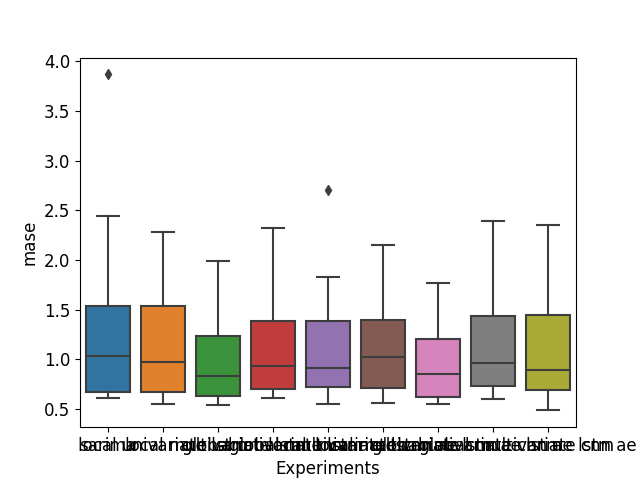
\includegraphics[width=\textwidth]{./figs/results/boxplot/mase-dataset_1.png}
  \hfill
  \caption{Boxplot of predictions made on dataset 1}
  \label{fig:results:boxplot-mase-dataset-1}
\end{figure}

\begin{figure}[h!]
  \centering
  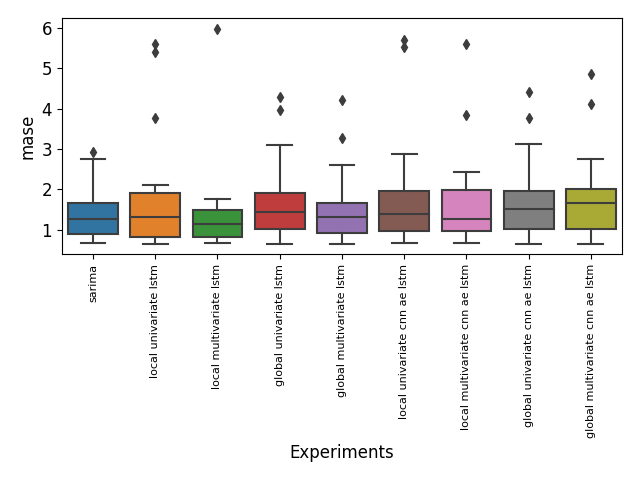
\includegraphics[width=\textwidth]{./figs/results/boxplot/mase-dataset_2.png}
  \hfill
  \caption{Boxplot of predictions made on dataset 2}
  \label{fig:results:boxplot-mase-dataset-2}
\end{figure}

\begin{figure}[h!]
  \centering
  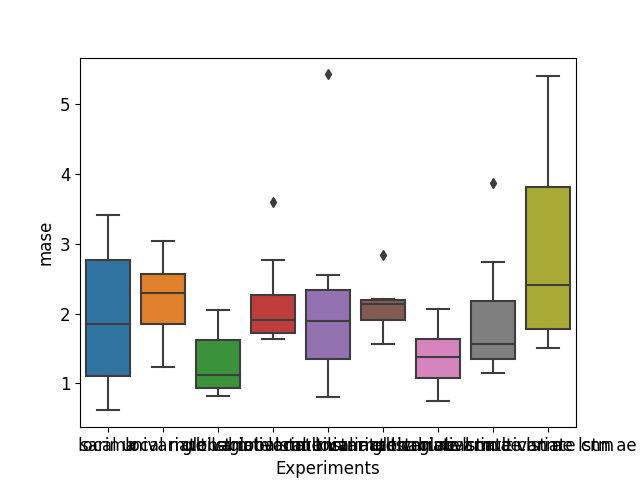
\includegraphics[width=\textwidth]{./figs/results/boxplot/mase-dataset_seasonal.png}
  \hfill
  \caption{Boxplot of predictions made on seasonal dataset}
  \label{fig:results:boxplot-mase-dataset-2}
\end{figure}

